\chapter{Evaluation}

\section{Experimental Results}

In this section, the proposed optimal control approach is implemented and its effectiveness tested and compared to the previous approach. The simulation setup is described in Sec. \ref{setup} and the results are shown in Sec. \ref{optimal control}. Sec. \ref{computation time} and Sec. \ref{performance guarantees} then focuses on the general performance of this new method in comparison to the previously used Scenario approach.

\subsection{Setup} \label{setup}

\subsection{Optimal Control with known basis functions} \label{optimal control}

\begin{figure}[htb]
\centering
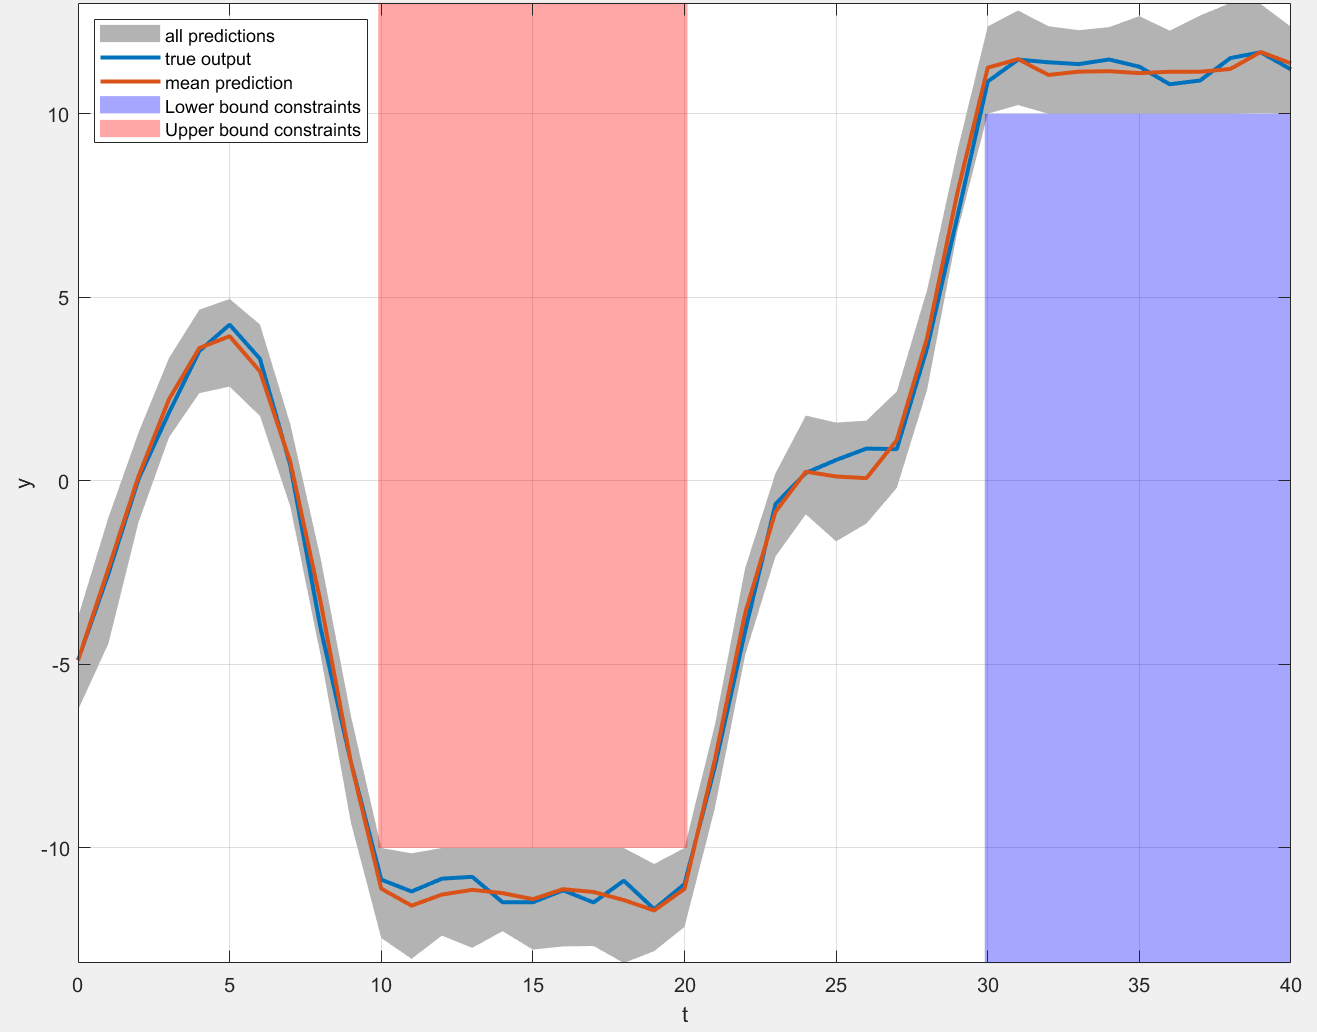
\includegraphics[width=0.6\textwidth]{pics/Scenario_plot.png}
\caption{Example velocity plot with units}
\label{fig:vel_plot}
\end{figure}

\begin{figure}[htb]
\centering
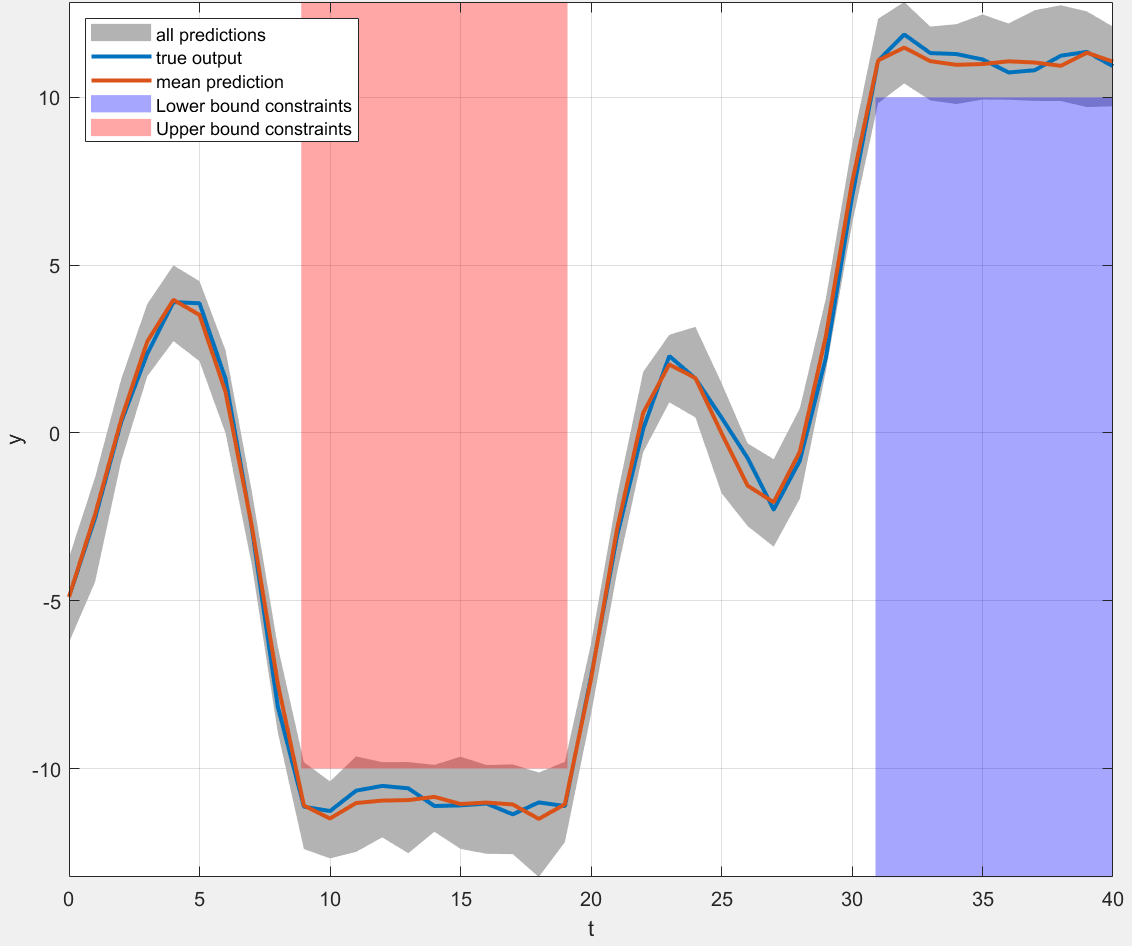
\includegraphics[width=0.6\textwidth]{pics/Kernel_plot.png}
\caption{Example velocity plot with units}
\label{fig:vel_plot}
\end{figure}

\begin{figure}[htb]
\centering
\subfigure[Subfigure 1 caption]{
   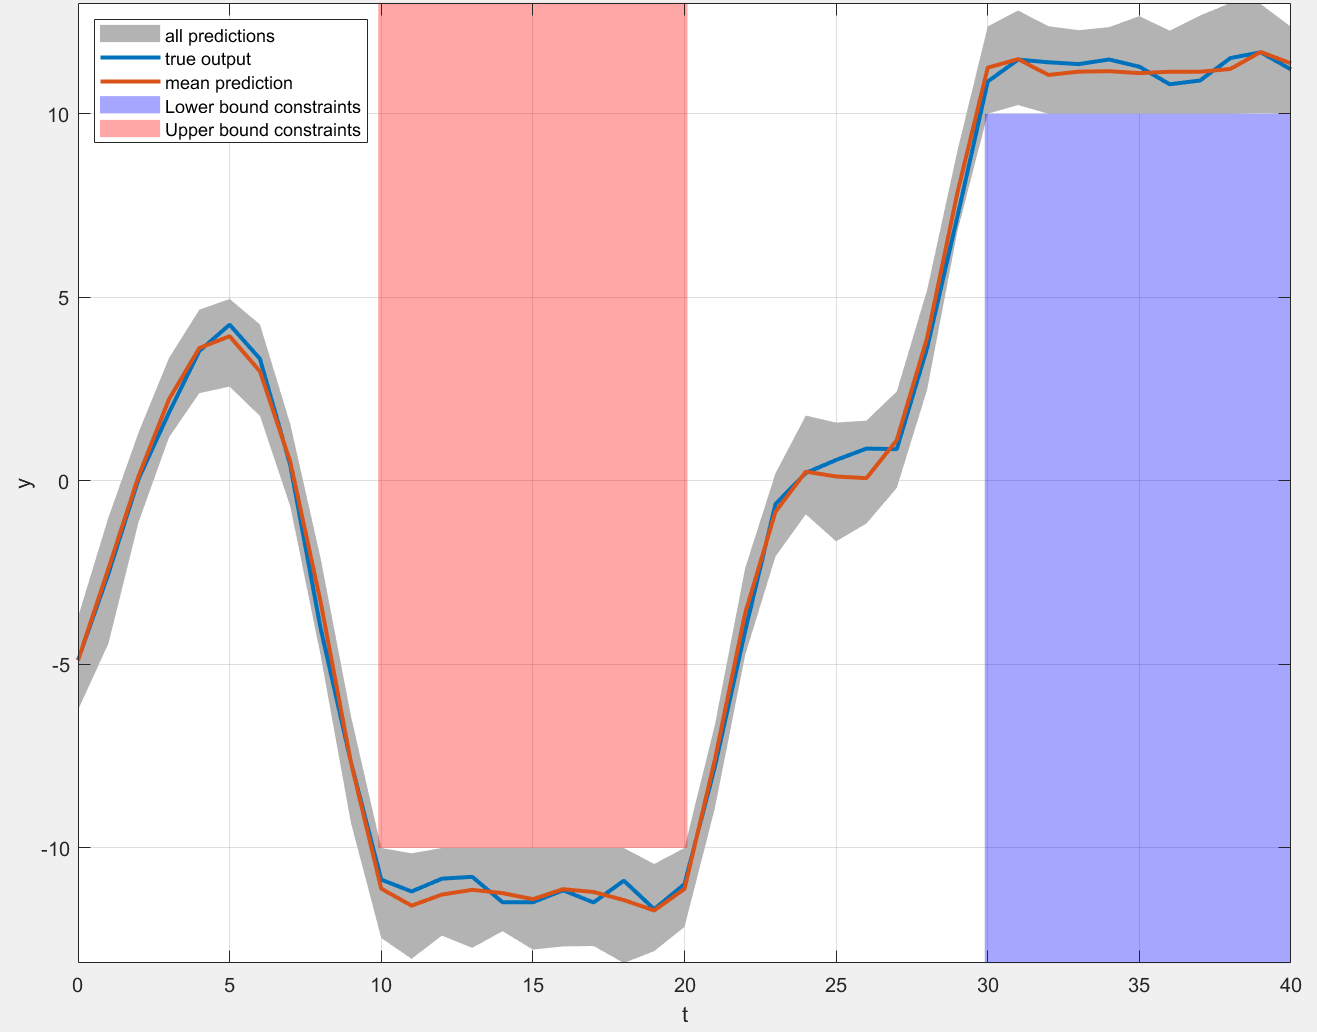
\includegraphics[width=0.3\textwidth] {pics/Scenario_plot.png}
   \label{fig:subfig1}
 }
\quad % puts next subfigure right next to the previous subfigure
\subfigure[Subfigure 2 caption]{
   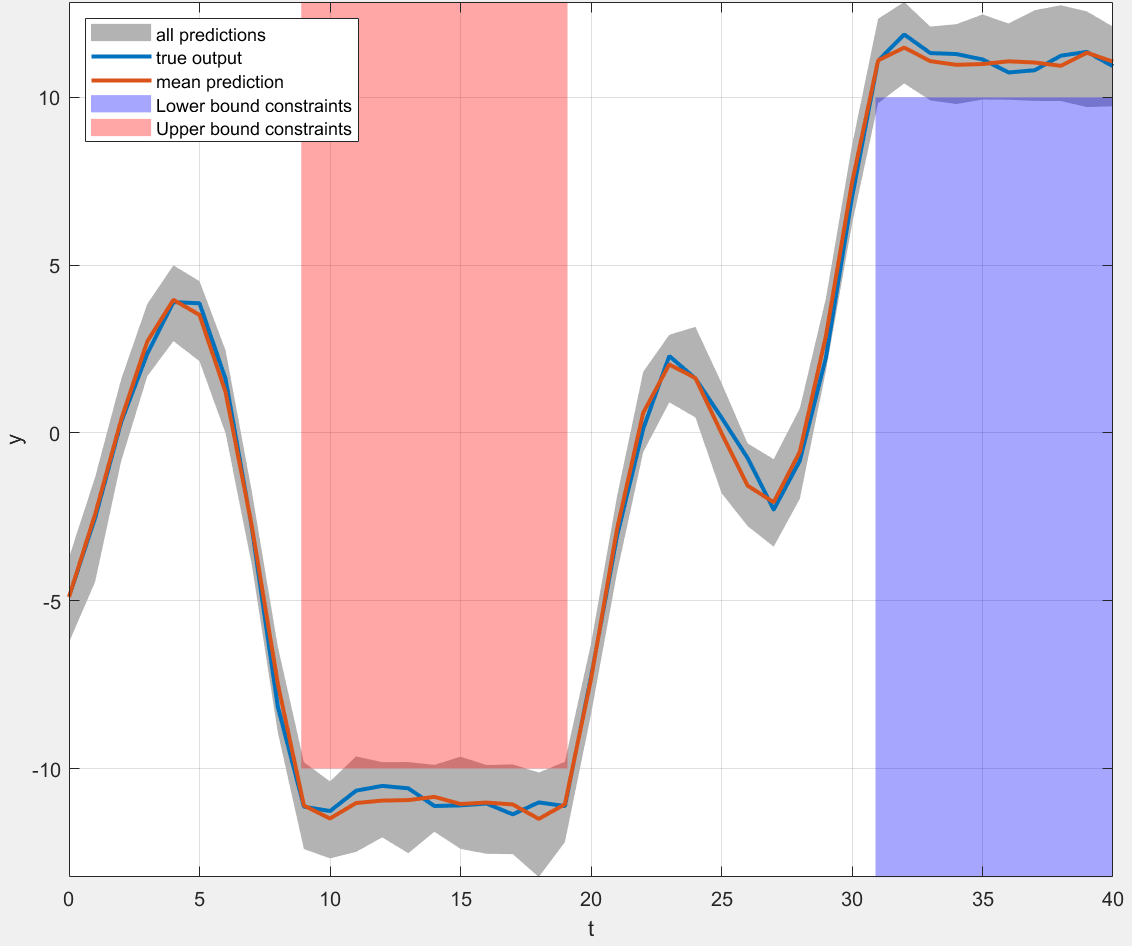
\includegraphics[width=0.3\textwidth] {pics/Kernel_plot.png}
   \label{fig:subfig2}
 }
\end{figure}

\subsection{Computation Time} \label{computation time}

\begin{figure}[htb]
\centering
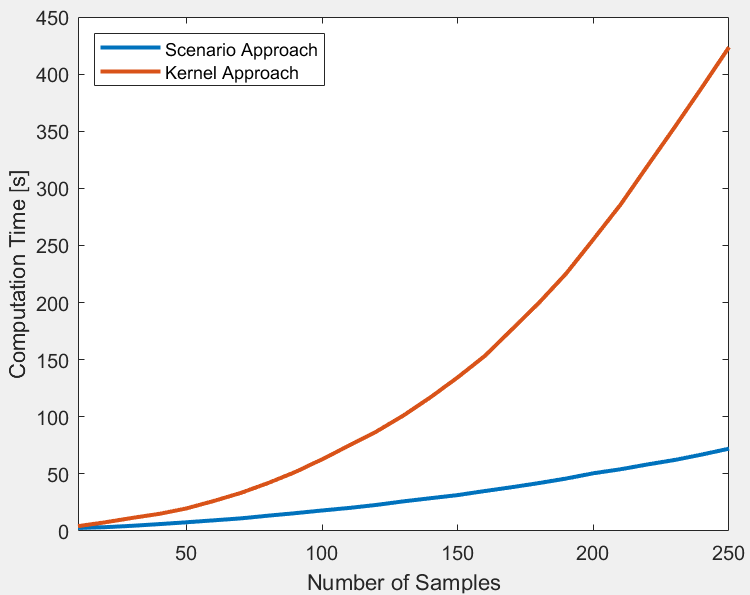
\includegraphics[width=0.6\textwidth]{pics/computationtime_plot.png}
\caption{Example velocity plot with units}
\label{fig:vel_plot}
\end{figure}

\subsection{Performance guarantees} \label{performance guarantees}

\begin{figure}[htb]
\centering
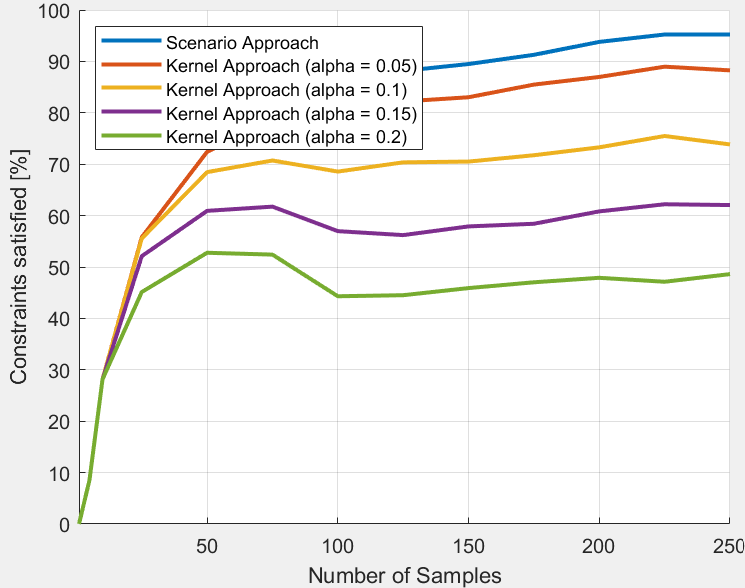
\includegraphics[width=0.6\textwidth]{pics/robustness_plot.png}
\caption{Example velocity plot with units}
\label{fig:vel_plot}
\end{figure}
 


